\documentclass[a4paper]{article}
\usepackage{latexsym,amssymb,amsmath,amsbsy,amsopn,amstext,xcolor,multicol}
\usepackage{ctex,hyperref,graphicx,wrapfig,fancybox,listings,subfigure}
\usepackage{pgf,pgfarrows,pgfnodes,pgfautomata,pgfheaps,pgfshade,tikz}
\usepackage[top=1in, bottom=1in, left=1.25in, right=1.25in]{geometry}
\graphicspath{{pic/},{draughts-server/}}
\title{\bf List of People in Wikipedia}
\date{2017.9}
\author{计64~~翁家翌~~2016011446}
\begin{document}
\kaishu
\ttfamily
\maketitle
%\tableofcontents
%\newpage
\section{软件用途}
本软件是一个人物检索系统,使用 Python 3.5.2 编写,后端使用 Django 1.11.5,实现了显示约2.3万个人物的信息以及检索功能。
\section{运行方式}

源代码位于 \url{https://git.thusaac.org/trinkle/List_of_people}。使用方法为

\begin{lstlisting}
    sudo pip3 install django
    python3 manage.py runserver
\end{lstlisting}

在浏览器中输入 \url{http://127.0.0.1:8000} 即可访问。
\section{功能介绍}
\subsection{主界面}

\begin{figure}[htp]
\centering
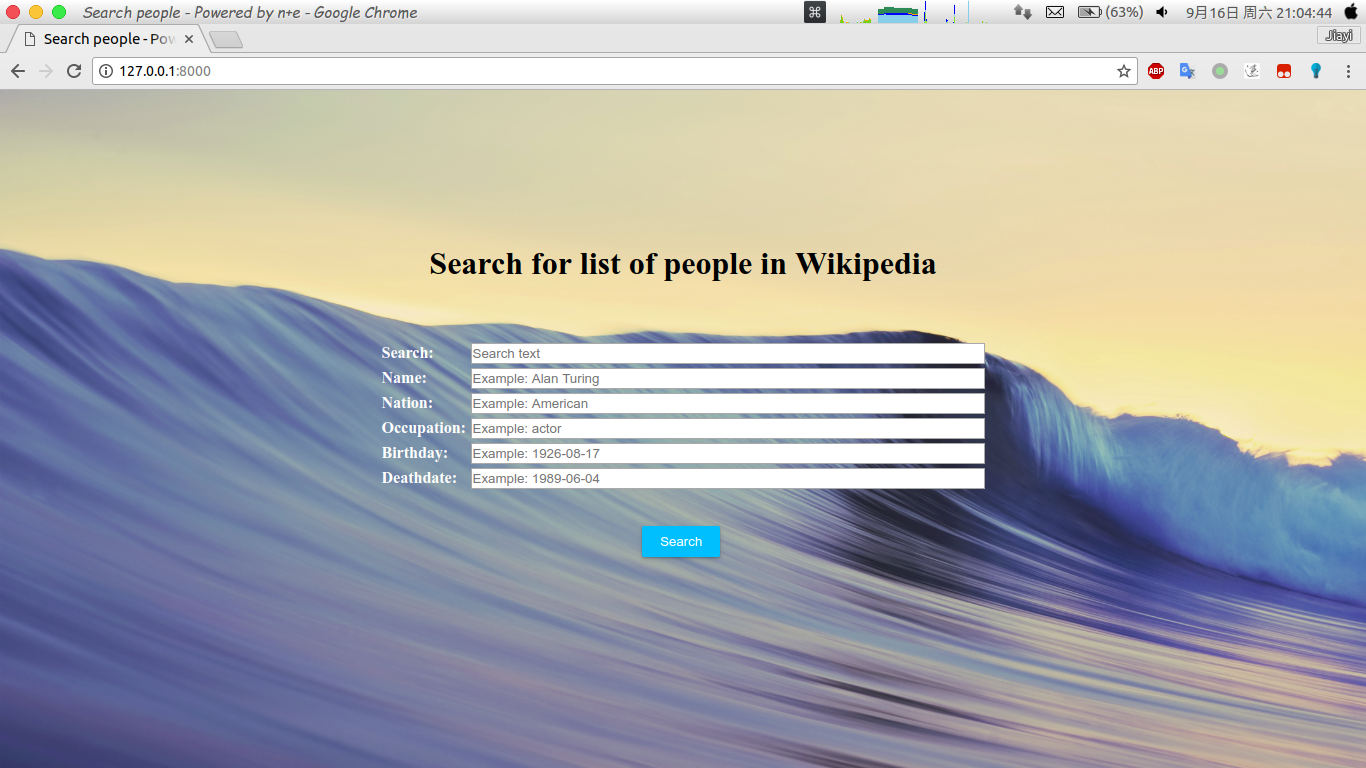
\includegraphics[width=1\linewidth]{main.png}
\caption{主界面}
\label{fig:start}
\end{figure}

图~\ref{fig:start} 显示了主界面。第一栏可以输入任意关键字,后面的五栏可以输入指定关键字进行匹配检索。点击 \fbox{Search} 即可进行搜索。

\subsection{搜索界面}
\begin{figure}[htp]
\centering
\includegraphics[width=1\linewidth]%{result.pdf}
{search.png}
\caption{搜索结果界面}
\label{fig:search}
\end{figure}

图~\ref{fig:search} 显示了输入关键词之后返回的查询结果页面,图中的查询关键字为 {\bf Name:} \uline{Andrew Yao}, {\bf Occupation:} \uline{Computer scientist}, {\bf Birthday:} \uline{1946-12-24}。搜索引擎会返回匹配程度最高的50条结果,如果关键词越多,定位也就越精确,搜索引擎会智能返回若干条最有用的信息。

\subsection{人物展示界面}

图~\ref{fig:yao} 显示了在点击图~\ref{fig:search} 第一个选项之后的界面,此时搜索引擎会在网页文本中高亮显示之前查询的关键字(黄色背景),并且刷新之后就会取消高亮。所有外部链接均能正常访问。此时访问页面会被标记为该人物的编号,并且在表格最下端会显示分类和编号。

图~\ref{fig:xjp} 显示了国家主席的页面,可以在网址的find后面直接输入姓名,即可跳转到对应人物的页面。

图~\ref{fig:comp} 显示了人物的完整页面。除了人物的信息显示之外,\fbox{Previous} 和 \fbox{Next} 两个按钮能够跳转页面到上一个/下一个人物,并且能够直接在最下端输入搜索信息进行搜索。

\section{程序实现}

爬虫使用 Python 的第三方库 BeautifulSoup 进行编写,位于 \uline{data/spd.py},每次将网页上的infobox所在的\uline{<table>}标签存入本地文件中,{\bf 不进行任何修改}。

得到原始数据之后,使用 BeautifulSoup 和 pickle 进行数据预处理,代码位于 \uline{data/preload.py},经过统计约有23000个有效的人物页面。处理后的数据保存为 \uline{data/cache.pkl}。

使用 Django 中,主体代码位于 \uline{find/views.py},每次将原始数据动态渲染,保存在 \uline{data/people.html} 中,并返回给 HttpRequest。

搜索算法为有效打分机制,如果匹配的关键字越多则分数越高,排名越靠前。

\begin{figure}[htp]
\centering
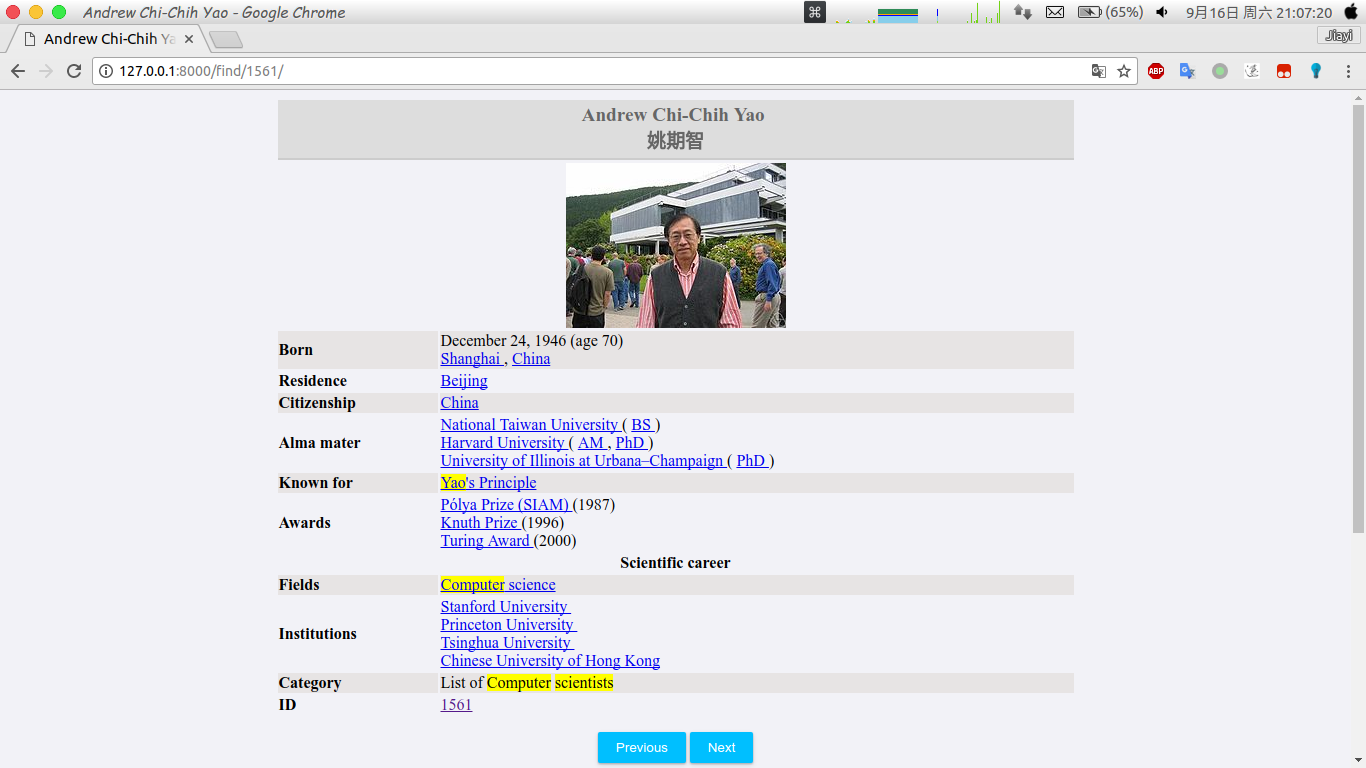
\includegraphics[width=0.98\linewidth]{yao.png}
\caption{Andrew Chi-Chih Yao}
\label{fig:yao}
\end{figure}

\begin{figure}[htp]
\centering
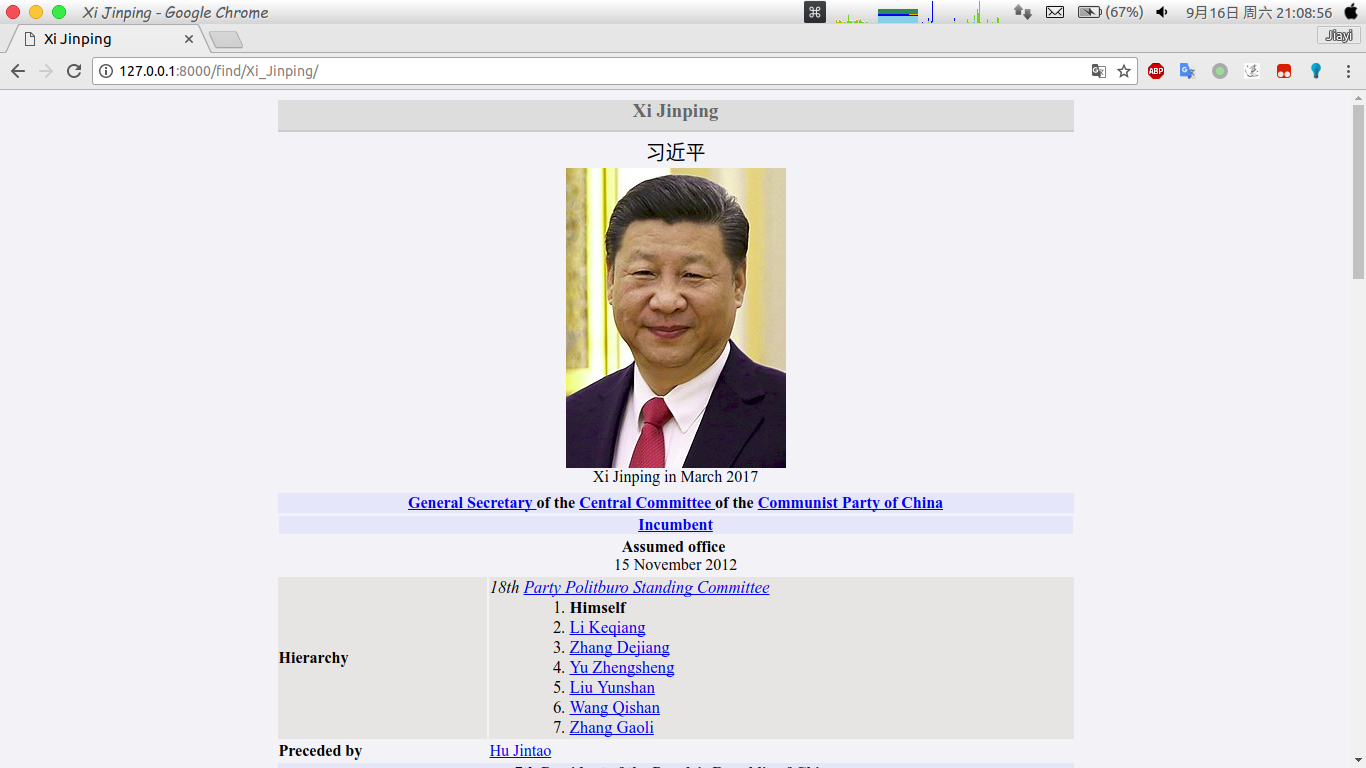
\includegraphics[width=0.98\linewidth]{president.png}
\caption{Xi Jinping}
\label{fig:xjp}
\end{figure}

\begin{figure}[htp]
\centering
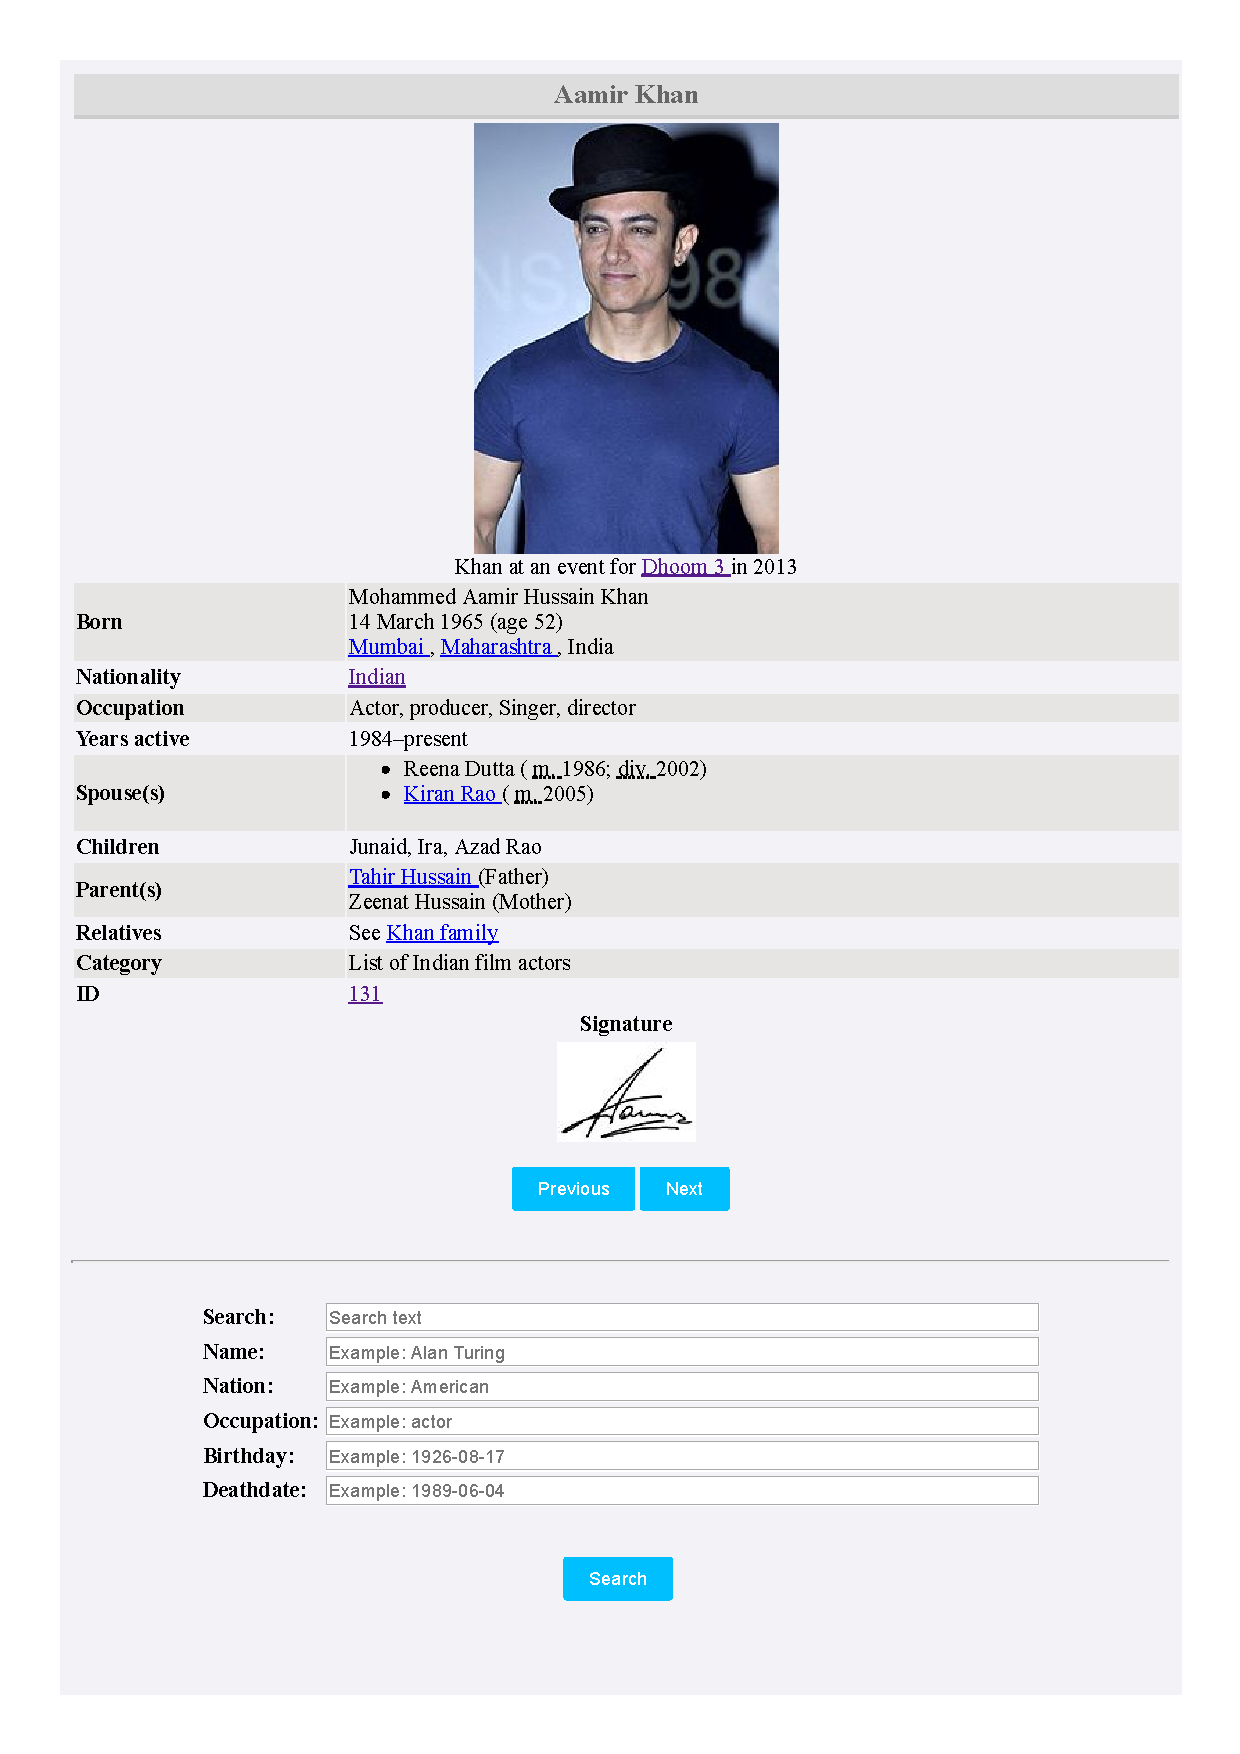
\includegraphics[width=1\linewidth]{Aamir_Khan.pdf}
\caption{Aamir Khan}
\label{fig:comp}
\end{figure}

\end{document}